\documentclass{standalone}
\usepackage{pgfplots}
\begin{document}
	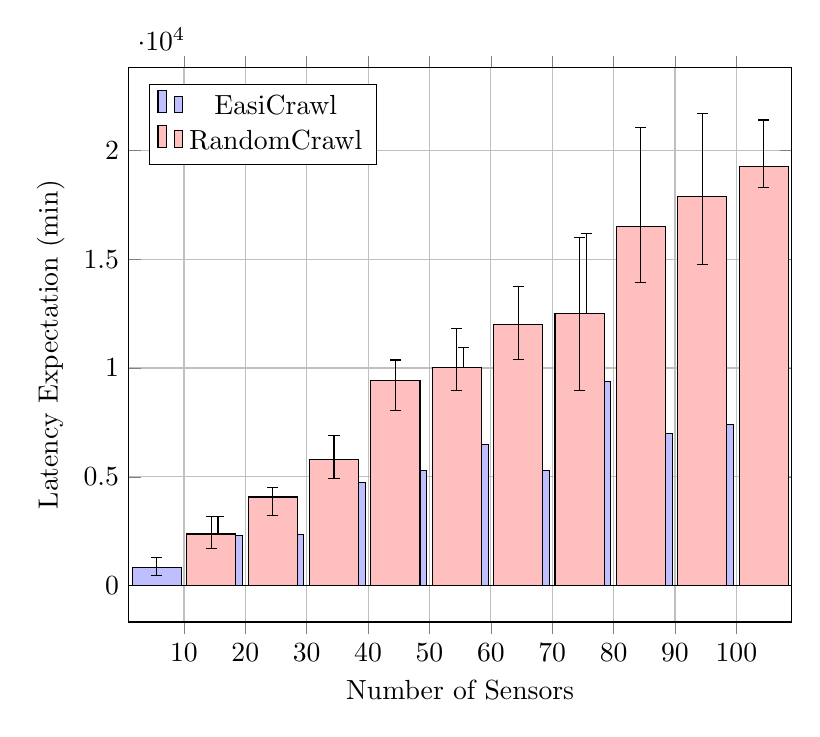
\begin{tikzpicture}
	\begin{axis}[
	% title = {Optimization based upon co-occurences},
	width=10cm,
	xtick={10,20,30,40,50,60,70,80,90,100},
	xticklabels={10,20,30,40,50,60,70,80,90,100},
	grid=major,
	ybar,
	bar width=8,
	ylabel= {Latency Expectation (min)},
	xlabel={Number of Sensors},
	legend pos= north west]
		
	\addplot[
		fill=blue!25,
		draw=black,
		point meta=y,
		every node near coord/.style={inner ysep=5pt},
		error bars/.cd,
		y dir=both,
		y explicit
	] 
	table [y error plus=y_max, y error minus=y_min] {
		x   y   y_max    y_min
		10	845 455 395
		20	2285	881	1182
		30	2330	959	937
		40	4726	501	335
		50	5289	2951	2176
		60	6484	4458	3280
		70	5278	4082	2735
		80	9379	6817	3613
		90	6998	3572	3714
		100	7412	1104	1405
	};
	
	\addplot[
	fill=red!25,
	draw=black,
	point meta=y,
	every node near coord/.style={inner ysep=5pt},
	error bars/.cd,
	y dir=both,
	y explicit
	]
	table [y error plus=y_max, y error minus=y_min] {
		x   y   y_max    y_min
		10	2369	786	670
		20	4071	448	850
		30	5809	1074	903
		40	9419	949	1373
		50	10014	1807	1068
		60	12011	1731	1610
		70	12492	3517	3512
		80	16510	4529	2581
		90	17899	3794	3130
		100	19248	2150	957
	};
	
	\draw ({rel axis cs:0,0}|-{axis cs:0,0}) -- ({rel axis cs:1,0}|-{axis cs:0,0});
	\legend{EasiCrawl,RandomCrawl};
	\end{axis}
	\end{tikzpicture}
\end{document}